% Chapter 4

\definecolor{MPLgreen}{RGB}{0,128,0}
\definecolor{MPLred}{RGB}{238,34,12}
\definecolor{MPLblue}{RGB}{31,119,180}

\chapter{How do Galaxies Acquire Mass? Assembly vs. Star Formation} % Write in your own chapter title
\label{Chapter:GalGrowth}
\lhead{Chapter 4. \emph{In-situ vs. Ex-situ growth}} % Write in your own chapter title to set the page header

\section{Background}
%What is insitu and exsitu growth
Galaxies acquire stellar mass in two ways, starformation and satellite accretion (mergers). Star formation is the process of gas collapse to form stars, galaxies at high redshift are thought to produce most of their mass through star formation. Star formation then reaches a peak at redshift $z=2$. The cessation (quenching) of star formation remains an open question, the leading theories involve a number of internal and external processes, from stellar and active galactic nuclei feedback to host halo and/or morphological quenching \citep{Granato2004AHosts, Dekel2009ColdFormation, Lilly2013GASHALOS, Schawinski2014TheGalaxies}. 

In contrast to star formation the assembly of mass though mergers is thought to increase at lower redshifts. In particular, in very massive galaxies growth via satellite accretion has been claimed to become progressively more relevant \citep{DeLucia2006TheGalaxies,vanDokkum2010THE2, Shankar2013SizeUniverse, Shankar2015, Buchan2016, Groenewald2017TheGrowth, Matharu2019HSTMergers}. Central galaxies that reside at the centre of massive haloes thus provide a window into the different pathways that have contributed to the mass growth history of galaxies in the local universe. Exploring the way these galaxies build their mass can give insights into the stellar-mass-halo-mass (SMHM hereafter) relation, the efficiency of the satellite transport from the edge of the cluster to the centre, the balance of the major processes taking place on these satellites, the galaxy merger rate, and the star formation rate. The characteristic mass at which galaxies transition from being in-situ to ex-situ growth dominated has previously been found at $M_* \sim 10^{11} M_{\odot}$ \citep{Cattaneo2011HowMass, Bernardi2011EvidenceRelations, Shankar2013SizeUniverse}. 

\subsection{Previous techniques}

Models of galaxy formation traditionally use the hierarchical growth of dark matter structure as the backbone for galaxy assembly. Hydrodynamical simulations co-evolve the dark matter and baryonic matter allowing for a simultaneous look at the assembly of both components \citep{McAlpine2015TheCatalogues,Vogelsberger2014IntroducingUniverse}. The latter technique, however, requires large computational resources. Less computationally intensive models such as traditional Semi-analytic and Semi-empirical models use dark matter merger trees from post-processing of dark matter simulations \citep{Guo2011FromCosmology, Shankar2013}. Dark matter merger trees visualize dark matter assembly as a central trunk and halo mergers happen where branches join. Semi-analytic models initialize gas at high redshift and use a number of physical assumptions and free parameters to tune to observations \citep{DeLucia2006TheGalaxies, Guo2011FromCosmology}. Semi-empirical models use a more direct approach initializing galaxy stellar mass in dark matter haloes most commonly through abundance matching, the association of galaxies to dark matter host haloes via relative abundances \citep{Hopkins2010MERGERSMATTER, Zavala2012, Moster2013, Shankar2014, Moster2018Emerge10}. Both Semi-Empirical and Semi-Analytic models follow the merging histories of the underling dark matter merger trees to track the in-situ and ex-situ buildup of galaxy mass. The work of \citet{Moster2018Emerge10}, for example, uses a semi-empirical model to associate the growth of the dark matter halo to the star formation rate of the host galaxy alongside the build-up of stellar mass from satellites accretion, further strengthening the connection between the dark matter host environment and the build-up of galactic stellar mass.


It is of relevance to the calculation of in-situ vs ex-situ mass buildup that the observed star formation rate is significantly higher than continuity estimates of the star formation rate \citep[e.g.][]{Leja2015ReconcilingFunction, Lapi2017StellarEquation}. It is consequently found that if observed star formation rates are used in models, they cannot be reconciled with the stellar mass functions. This is a particular problem for semi-empirical models where one would ideally use the observed star formation rate as an input. To overcome the inconsistencies between observed star formation rates and model predictions it is possible to include continuity star formation rates. Attributing the stellar mass growth to star formation in this way yields an upper limit to star formation rate that is consistent with the stellar mass function evolution by design true to the empirical approach.


\section{Constraining the In-Situ vs. Ex-Situ growth in \steel}
%methods and importance of constrained histories
To properly constrain the formation of a galaxy one must reproduce the galaxy environment, the distribution of satellites around the central galaxy, at all previous redshifts. Discrepancies with observations of the the high redshift environment will cause modelled satellite stellar mass accretion rates that are either too high or too low. To account for such deficit/surplus modelled in-situ growth must compensate though other modelling parameters to maintain the evolution of the stellar mass density. Such compensation could, for example, be of the form of suppressed/enhanced star formation rate or alternatively an any number of other physical modelling parameters. Reproducing the number density and distribution of galaxies has however proven a challenge for many semi-analytic models \citep[e.g.][]{Asquith2018CosmicModels}. Furthermore, where semi-analytic models have included more physics via an increased number of modelling parameters, this has led to degeneracies that obscure which are the essential physical processes governing galaxy formation \citep[e.g.][]{Lapi2011Herschel-atlasGalaxies,Gonzalez2011Evolution4}.

%following populations 

\section{Incompatible \LCDM and Stellar Mass Functions}
%Cartoons and methodology
The cartoon in Figure \ref{fig:SMFtoAcc} shows a simple visualization of the process we use to determine the effect of different stellar mass functions/SMHM relations on the accretion histories and thus ex-situ growth, of galaxy populations. Starting on the left we show two stellar mass functions, the primary difference is the blue (dotted) stellar mass function has a substantially enhanced high mass end. In the middle panel we show how this high mass slope changes the SMHM relation, an enhanced high mass end stellar mass function results in an enhanced high mass slope. The galaxy growth histories, shown as solid lines, are generated using the SMHM relation used to calculate the average satellite stellar mass accretion associated to a given central halo mass history.
It follows that the galaxy grown using the steeper relation from the enhanced stellar mass function induces more galaxy growth. A flatter high mass slope induces less growth for a flat slope the central galaxy would not grow with increasing halo mass.

\begin{figure}[h]
	\centering
	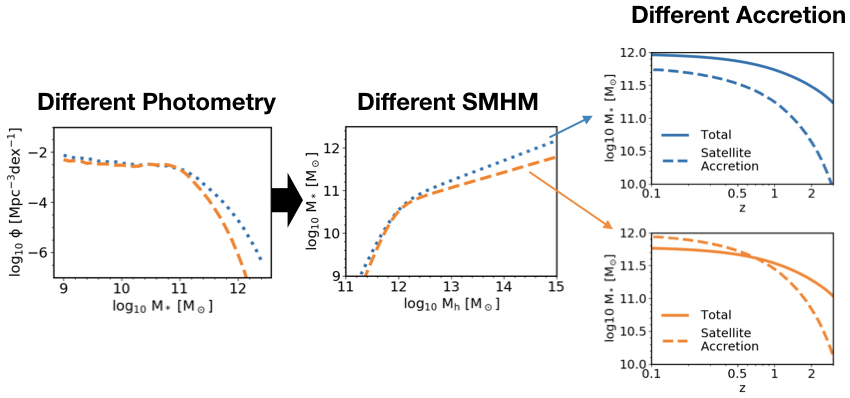
\includegraphics[width = \linewidth]{Figures/Chapter4/SMFtoAccretion.jpeg}
    \caption{A cartoon showing the steps we follow to connect the differences found in the stellar mass function (left) and the changes in the SMHM relation (SMHM, middle), that propagate into changes in the accretion histories (right). In the right hand panel dashed lines are mass from satellite accretion and solid lines are total galaxy mass growth. Flatter SMHM relations imply a weaker growth of stellar mass in the central which can be easily overcome by the substantial cumulative growth of merging satellites, rendering the model internally inconsistent.}
	\label{fig:SMFtoAcc}
\end{figure}

%cmodel
In Figure \ref{fig:SatelliteAccretioncMod} we show the satellite accretion generated using the `cmodel' SMHM relation/SMF given in Section \ref{C2:SubSec:AbnMtch}. 
The top row of  shows the total mass of the galaxy and the total contributed by satellite accretion. The middle row shows the fractional contribution from satellite accretion from $z = 3$. The bottom row shows the instantaneous mass growth from satellite accretion. In Figure \ref{fig:SatelliteAccretioncMod} we obtain a lower limit for the accretion rate by including stripping but not star-formation in the satellites thus minimizing their mass through environmental processes. We find for the high mass galaxies, which are above the knee of the SMHM relation, even the lower limit for the accretion has an instantaneous rate greater than the growth rate of the galaxy as seen in the bottom row. This makes the cmodel SMHM relation used within our dark matter accretion model \textit{non-physical}.

\begin{figure*}[h]
	\centering
	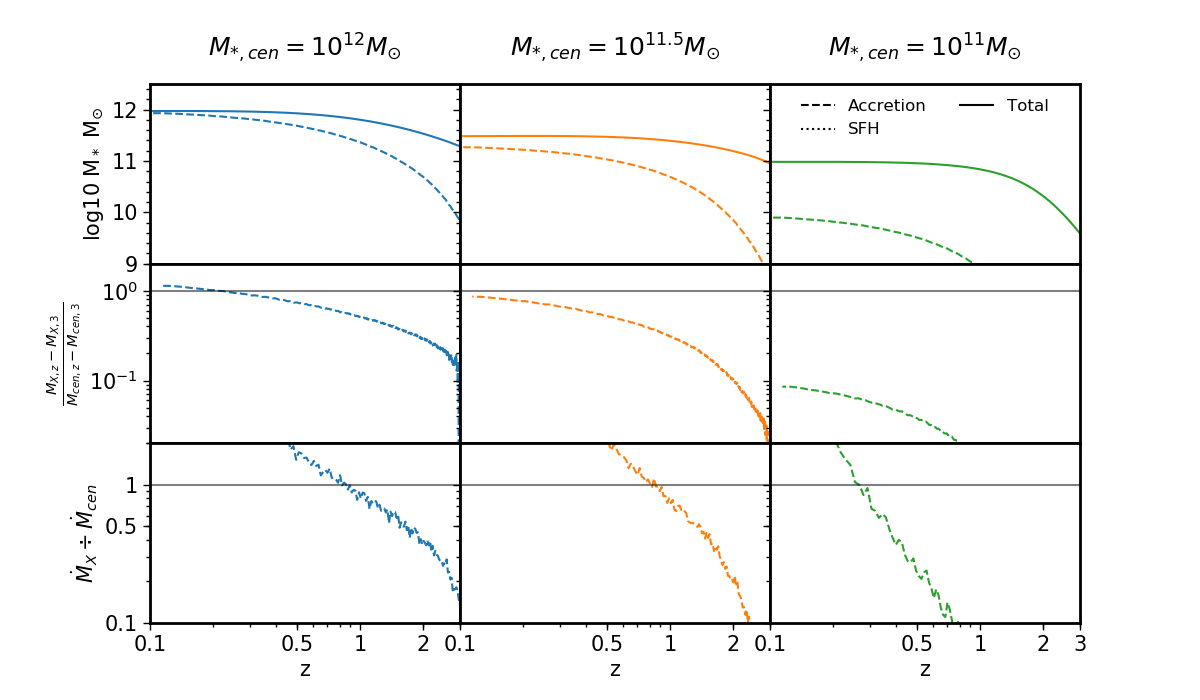
\includegraphics[width = \linewidth]{Figures/Chapter4/SatelliteAccretion_cMod.png}
    \caption{Three `mass tracks' are shown that have central galaxy masses at redshift $z = 0.1$ of $M_{*,cen}$ = $10^{12}$, $10^{11.5}$, and $10^{11}$ $[M_{\odot}]$ in blue orange and green respectively. It is clear that this model is internally nonphysical as the accretion via satellites (dashed lines) rapidly overshoots the total growth in stellar mass (solid lines) implied by the underlying growth host halo growth, as evident in the middle and bottom rows.}
	\label{fig:SatelliteAccretioncMod}
\end{figure*}

%pymorph
Similarly, the relative contributions to the average stellar mass growth of central galaxies from satellites and star formation history are calculated from \textsc{steel}, using the PyMorph SMHM relation/SMF given in Section \ref{C2:SubSec:AbnMtch}. This is shown in Figure \ref{fig:SatelliteAccretion} for three galaxy mass bins ($10^{11}$,$10^{11.5}$,$10^{12}$ $M_{\odot}$) selected at $z = 0.1$, the average growth history (total, solid lines) is derived by following the host halo-mass track, and the stellar-mass track is implied by imposing abundance matching at all redshifts. The stellar mass history assigned by abundance matching, is naturally independent of any galaxy merger modelling assumptions from \textsc{steel}. The total accretion from satellites (accretion, dashed lines) is computed from the expected satellite accretion along halo mass tracks. For each galaxy a star formation history (SFH, dotted lines) may then be calculated. The star formation rate is tuned such that it provides the correct star formation history to account for the difference between the mass growth expected from abundance matching and the cumulative satellite stellar mass accretion, the method for this is explained in detail in Section \ref{sec:SFR_Dev}.

\begin{figure}[h]
	\centering
	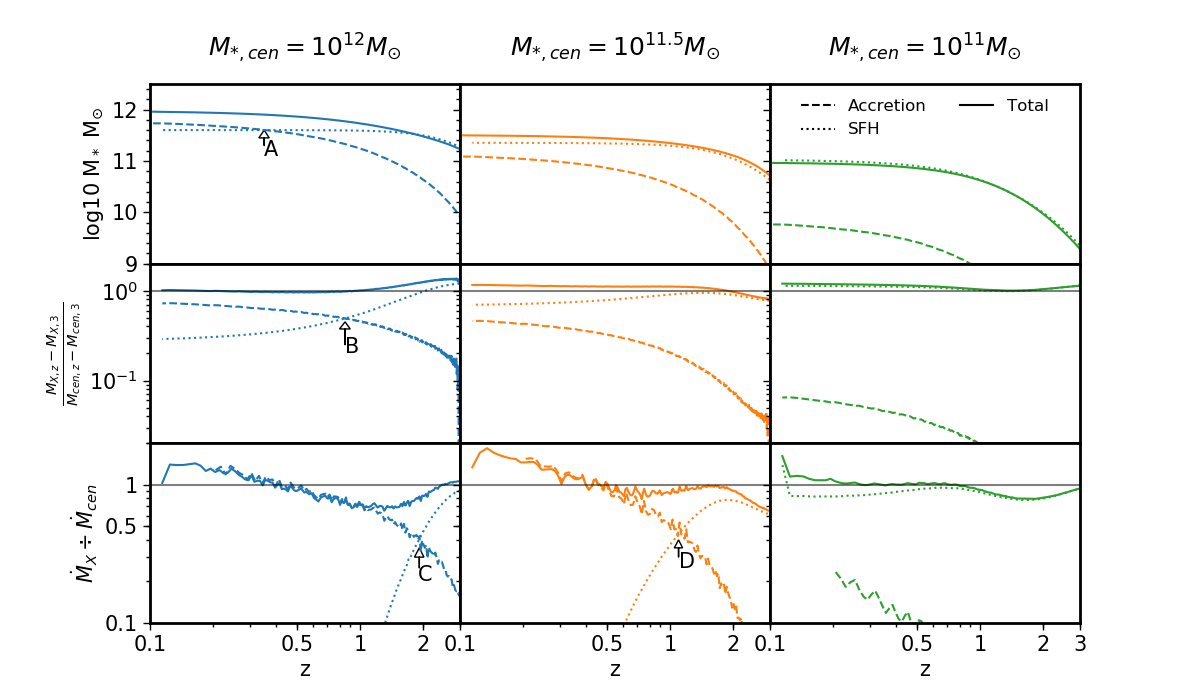
\includegraphics[width = \linewidth]{Figures/Chapter4/SatelliteAccretion_G19.png}
    \caption{Three `mass tracks' are shown that have central galaxy masses at redshift $z = 0.1$ of $M_{*,cen}$ = $10^{12}$, $10^{11.5}$, and $10^{11}$ $[M_{\odot}]$ in blue orange and green respectively. The satellite galaxy accretion is shown for evolved satellites with a dashed line, and the mass from star formation shown with a dotted line. The top panels show the total mass of the central (solid lines) and the total mass gained from accretion or star formation. The middle panels show the fraction of the total galaxy mass formed from satellite accretion or star formation since redshift $z=3$. The bottom panels show the ratio of the mass accretion rate from satellite galaxies, the star formation rate, and the mass growth rate of the central galaxy predicted by abundance matching. The black horizontal lines in the second and third rows are at unity. The solid lines showing the sum of the other two factors should be close to or on the unity lines. The labels A \& B point to where the cumulative mass from accretion overtakes the cumulative mass from star formation. The labels C \& D point to where the instantaneous accretion overtakes the star formation rate.}
	\label{fig:SatelliteAccretion}
\end{figure}

In Figure \ref{fig:SatelliteAccretion} we identify the epoch after which a galaxy transitions into a merger-dominated state under two definitions. Firstly, we define the ``cumulative transition'' as when the galaxy has accreted more mass than it has created from star-formation processes (Points A \& B). Secondly, we define the ``instantaneous transition'' as  the epoch when the growth rate from mergers overtakes the growth rate from star-formation (Points C \& D). More massive galaxies transition earlier to merger dominated growth under both definitions. However, all galaxies transition earlier under the second (instantaneous) definition. The masses shown in Figure \ref{fig:SatelliteAccretion} show three cases of relevant galaxy accretion tracks. The $M^{z=0}_* = 10^{12} M_{\odot}$ galaxy growth curve at low redshift is always dominated by satellite accretion. In the top and middle rows we see that more mass has been accreted than produced by star formation, and in the bottom row we see the accretion rate overtook the star formation rate at redshift $z=2$. The $M^{z=0}_* = 10^{11.5} M_{\odot}$ galaxy growth curve has more mass created from star formation than satellite accretion. However, the galaxy population has a higher rate of accretion rate than star formation rate since redshift $z = 1$. The final population shown at $M^{z=0}_* = 10^{11} M_{\odot}$ is star formation dominated under both cumulative and instantaneous definitions. At redshift $z = 0$ we find the transition masses for the total mass ratio and the instantaneous ratio to be at $M_* = 10^{11.7} M_{\odot}$ and $M_* = 10^{11.1} M_{\odot}$ respectively.

\section{Deriving the Star Formation Rate}
\label{sec:SFR_Dev}

The cartoon in Figure \ref{fig:SFRDerevation_Cartoon} shows the processes we follow to derive the star formation rate by following galaxy populations along their halo mass histories. \textcolor{MPLgreen}{The plot labelled 1 (green) is the input stellar mass function.} \textcolor{MPLred}{The box in red is the statistical dark matter accretion history described in Section \ref{subsec:SDMAH}, including the halo mass function (2a), the central growth histories (2b), and the halo substructure (2c) shown here as a discrete merger tree for visualization purposes.} Using the abundance matching routines described in Section \ref{C2:SubSec:AbnMtch}, the \textcolor{MPLgreen}{stellar mass function (1)} and the \textcolor{MPLred}{halo mass function (2a)} are used to create the SMHM relationship (3, black).


In Chapter \ref{Chapter:GalDist} we showed how the \textcolor{MPLred}{dark matter accretion histories (2)} and abundance matching (3) can be used to generate \textcolor{MPLblue}{distributions of satellites for any central halo at multiple redshifts (4)}. For each \textcolor{MPLred}{central halo mass track (2b)} we calculate the average number density of satellites that reach the center of the halo and merge with the central galaxy \textcolor{MPLblue}{thus generating the average satellite accretion history (dashed line, 5)}. \textcolor{MPLred}{Using the central halo growth histories (2b)} and the SMHM relation (3), we can generate the \textcolor{MPLblue}{average central galaxy growth history (solid line, 5)}. These two quantities can be compared to check for self-consistency, as described above and shown in Figure \ref{fig:SMFtoAcc}. Where a self-consistent central growth and accretion history is found any deficit between the accreted mass and the growth history is attributed to \textcolor{MPLblue}{star formation rate (delta, 5)}. \textcolor{MPLblue}{The derived star formation rate for central galaxies (solid line, 6) is compared to observational data (points, 6)}. Where the star formation rate prediction generated form the model is found to be consistent with observed star formation rates this is a good indication that the model is predicting correct accretion histories.

%Big Cartoon
\begin{figure}[h]
	\centering
	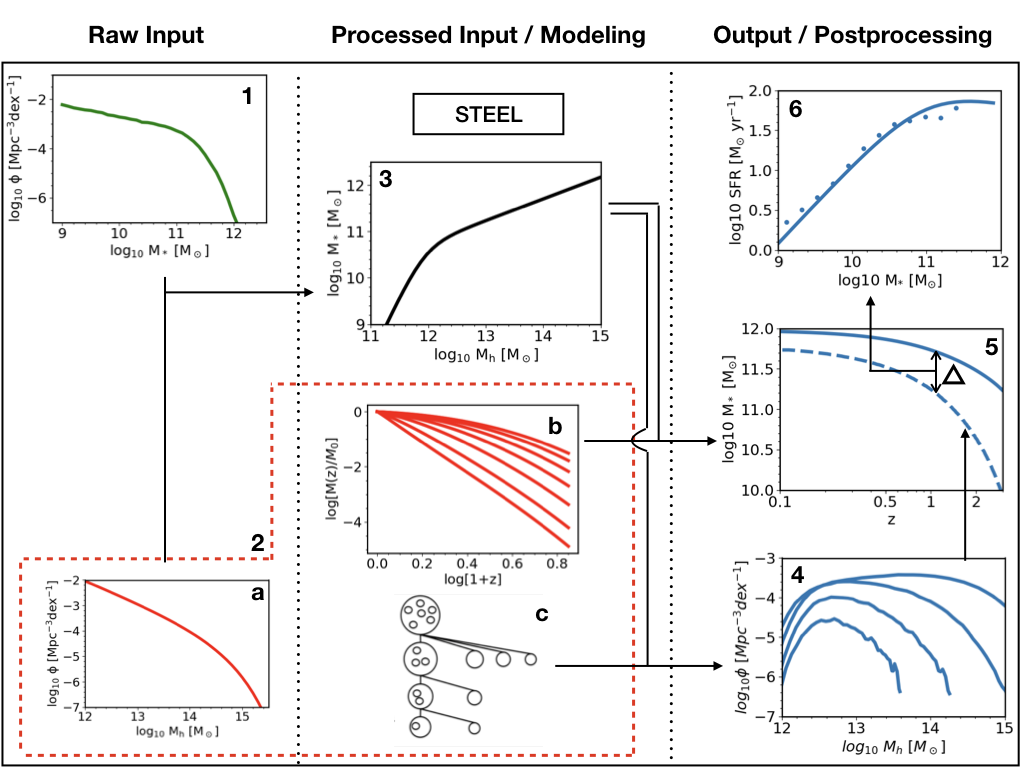
\includegraphics[width = \linewidth]{Figures/Chapter4/SFRFullCartoon.png}
    \caption{A cartoon showing the constituent steps of the method to generate star formation rates. In brief, the three columns from left to right are raw inputs, derived inputs/modelling, and output/post-processing. The subplots are: 1. The stellar mass function, 2a. The halo mass function, 2b. Halo mass growth histories, 2c. Accretion histories/Merger tree, 3. The SMHM relation, 4. Group/Cluster satellite richness, 5. Central growth histories/satellite accretion histories, 6. Star formation rate. The star formation rates are derived from the difference between the total growth in stellar mass and that from satellite accretion (panel 5).}
	\label{fig:SFRDerevation_Cartoon}
\end{figure}

The method described above directly links the star formation rate to the accreted mass from satellites. However, in our model satellites grow in mass after infall, we therefore must recalculate the full satellite accretion onto the central galaxies updating their mass using the new star formation rate. Using the updated accretion the star formation rate is recalculated beginning an iterative process. However, this iterative process of recalculation ends after one loop as the re-derived accretion is found to be nearly identical, as expected from the results of Chapter \ref{Chapter:GalDist}. When calculating this difference we also take into account the stellar mass loss rate (MLR) due to stellar recycling using Equations \ref{eqn:f_ml} \& \ref{eqn:MLR}. The star formation rate - stellar mass relation derived from this method is fit with a double power law that evolves with redshift given by the following Equation \ref{eqn:SFR_DPL},
\begin{equation}
\label{eqn:SFR_DPL}
\begin{split}
SFR(M_*, z) &= 2N(z)\Big[ \Big( \frac{M_*}{M_{n}(z)}\Big) ^{- \alpha(z)} + \Big( \frac{M_*}{M_{n}(z)}\Big)^{\beta(z)} \Big ]^{-1}\\
\log_{10} N(z) &= 10.65 + 0.33z - 0.08z^2\\
\log_{10} M_{n}(z) &= 0.69 + 0.71*z - 0.088z^2\\
\alpha(z) &= 1.0 - 0.022z + 0.009z^2\\
\beta(z) &= 1.8 - 1.0*z - 0.1z^2.
\end{split}
\end{equation}

\begin{figure}[h]
	\centering
	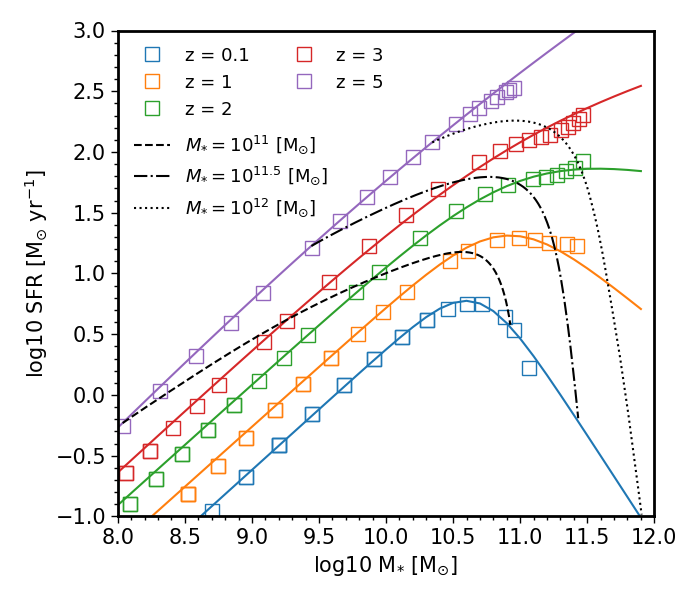
\includegraphics[width = 0.8\linewidth]{Figures/Chapter4/HMC_DPL.png}
    \caption{The star formation rate - stellar mass relation derived from following central galaxy populations along halo mass histories at redshifts $z = 0.1, 1, 2, 3, 5$. The data extracted from the post-processing of \textsc{steel} are shown by coloured crosses and the double power-law fits are shown as lines in corresponding colours. The three black lines are the evolution of the galaxy populations selected at redshift $z=0.1$ with masses $M_* = 10^{11}, 10^{11.5}, 10^{12} [M_{\odot}]$  presented in Figure \ref{fig:SatelliteAccretion}.}
	\label{fig:SFR_DPL}
\end{figure}

This fit (solid lines) to the computed SFR (open squares) is shown in Figure \ref{fig:SFR_DPL}. When visualised the general trend of the SFR is at lower redshift: the normalization decreases, the peak of the distribution shifts to lower masses, and the turnover after the peak is steeper. We also show the same three galaxy population tracks from Figure \ref{fig:SatelliteAccretion} as black lines. These tracks show how the galaxy population evolves in SFR with redshift. The population tracks show a gradual increase in SFR and then a turnover before dropping sharply, as they transition to a satellite accretion-dominated regime. It is found that smaller galaxies grow for longer timescales with increasing star formation, whilst larger galaxies start with higher star formation rate and transition to an accretion-dominated phase much earlier in time.

%Match to panchromatic data
\begin{figure}[h]
	\centering
	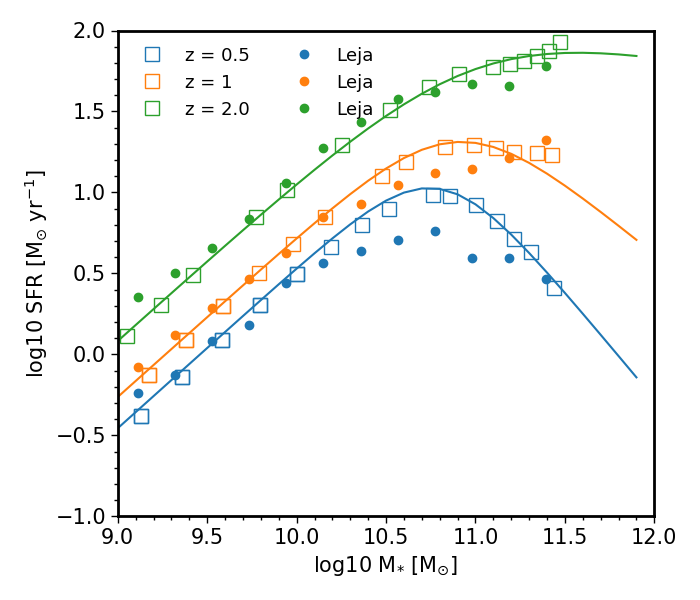
\includegraphics[width = 0.8\linewidth]{Figures/Chapter4/HMC_DPL_wLeja.png}
    \caption{I show the star formation rate - stellar mass relationship from Figure \ref{fig:SFR_DPL} at redshifts z = 0.5, 1, 2 (blue orange and green respectively, \textsc{steel} data are crosses and fits are solid lines). In this plot we compare with the observed star formation rate from \citet{Leja2019AnSurvey} shown as filled circles with corresponding colours denoting corresponding redshift.}
	\label{fig:SFR_L18}
\end{figure}

Recent work, where the star formation histories are properly accounted for when measuring star formation rates, has suggested that the previous determinations of star formation rates using UV+IR are 0.1 to 1 dex too high \citep{Leja2019AnSurvey} and cannot be reconciled with the growth of the stellar mass function \citep{Leja2015ReconcilingFunction, Lapi2017StellarEquation}. Our star formation rate is consistent with the results of \citet{Leja2019AnSurvey}, as reported in Figure \ref{fig:SFR_L18}. The excellent match to Leja et. al.'s independent estimates further supports the idea that a more robust method to derive more reliable star formation rates is to follow galaxy assembly along host halo growth histories \citep[see e.g.,][]{Moster2018Emerge10}. 

\subsection{Specific Star Formation Rate Distribution}
\label{subsec:sSFR}

Figure \ref{fig:sSFR} shows the specific star formation rate distribution of satellites in three mass ranges, as labelled, chosen to probe transitions found in observational data \citep{Bernardi2011EvidenceRelations, Bernardi2014SystematicMorphology, Cappellari2013TheFunction}. The solid blue line and the dashed black lines show the satellite and central sSFR from \textsc{steel}, respectively, while the grey histogram shows the satellites from SDSS and the unfilled histogram shows the centrals in SDSS. 

\textsc{steel} accurately captures the key trends in the distributions, such as bimodality, which is seen in both the central and satellite populations. The central population below $M_{*} = 10^{10.5}$ [M$_{\odot}$] is mostly star-forming whereas the satellites show signs of quenching. In the intermediate-mass range a fraction of the centrals become quenched and the satellites show a strong quenching effect. In the highest mass range all galaxies show strong quenching features with little star-formation. Whilst still not an exact match to the SDSS distribution, we find that including a redshift dependence in the dynamical quenching provides a better fit than the model used in Paper \RomanNumeralCaps{1}. The central sSFR is calculated using the star formation rate presented in Figure \ref{fig:SFR_DPL}, which uses the PyMorph SMHM relation. Each central mass is assigned a star formation rate with a scatter of 0.2 dex. To account for the fraction of galaxies that are quenched via mergers at each stellar mass we modify the assigned star formation rates by setting a fraction of galaxies equal to the elliptical fraction to have a sSFR of $10^{-12}$ [$yr^{-1}$] with a scatter of 0.2 dex and in turn increase the star formation rate of the remaining galaxies to maintain the same average star formation rate for the population. This approach tests if mergers alone can account for the bimodality found in the central sSFR, the high mass centrals $ > 10^{11.3}$ [M$_{\odot}$], but produces an inadequate fit to the SDSS centrals at masses lower than $10^{10.5}$ [M$_{\odot}$]. The discrepancies in the location of the star-forming population are likely caused by the imperfect fit to observed SFR as seen in \ref{fig:SFR_L18} and the deficit of quenched galaxies in the lower mass cuts is likely due to causes of quenching that are not merger related (e.g., AGN feedback).

%How the quenching differs
\begin{figure}[h]
	\centering
	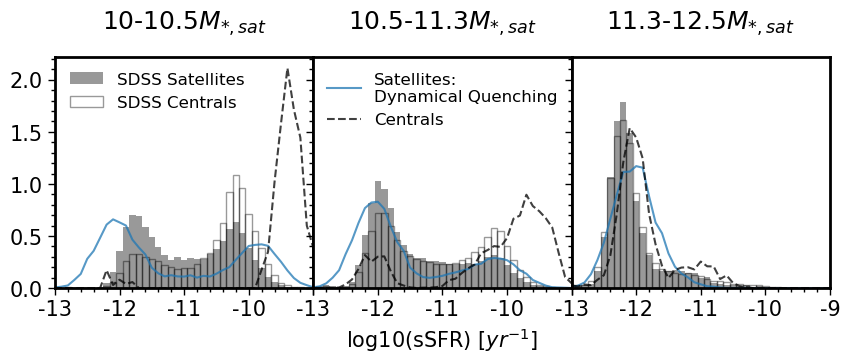
\includegraphics[width = \linewidth]{Figures/Chapter4/SSFR.png}
    \caption{We show the sSFR of satellites and centrals compared to SDSS in three mass bins selected to mirror proposed breaks in the galaxy main sequence. The SDSS data for satellites and centrals are filled and unfilled histograms respectively. The \textsc{steel} result for the satellites is the solid blue line and the post processed central result is the dashed black line.}
	\label{fig:sSFR}
\end{figure}

\section{Discussion}

In this chapter we found one of the major factors in regulating the in-situ and ex-situ accretion pathways to be the \textit{shape} of the SMHM relation. A shallower low-mass slope causes larger amounts of satellite accretion as smaller haloes, with much higher number density, are initialized with larger satellite galaxies. Similarly to \citet{Shankar2006NewFormation} \& \citet{Moster2018Emerge10}, we find the high mass slope to undergo only a small amount of evolution with increasing redshift, this implies the growth of central galaxies is directly linked to the steepness of the high mass slope and the growth of the host halo. The flatter the high mass slope of the SMHM relation, the less growth is expected in stellar mass following the assembly of the host dark matter halo. In turn, a weak evolution in the stellar mass content of the central galaxy can be in tension with what is expected from satellite accretion, especially for the most massive galaxies. We discussed that the slope of the high-mass end of the stellar mass function and implied slope of the SMHM relation strongly depend on the choice of light profile, background subtraction, and mass-to-light ratios. However, not all resulting stellar mass functions provide physically self-consistent results in a LCDM Universe. Steeper SMHM relations, such as those predicted by PyMorph-based stellar mass functions \citep{Bernardi2013TheProfile}, produce more consistent central and satellite accretion stellar mass growths. In addition to models with different SMHM slopes, we also tested models with the dynamical time varied by $\pm$20$\%$, within the range of possible dynamical times predicted in Chapter \ref{Chapter:GalDist} constrained by satellite richness. This relatively modest alteration has a minor effect on the satellite accretion rate and mass contribution to the central. In this work we find the transitional stellar mass, above which dry mergers progressively become the major contributor to galaxy growth, to be $M_{*} = 10^{11.1}$, see Figure \ref{fig:SatelliteAccretion}. The latter is consistent with previous findings \citep[e.g.,][]{Bernardi2011EvidenceRelations, Cappellari2013EffectEvolution, Shankar2013SizeUniverse}.


By following the statistical dark matter accretion histories we were able to use the central mass tracks and abundance matching to obtain a growth history for central galaxies. Subtracting from the latter at each time step the cumulative stellar mass from satellite accretion, we created a `star formation rate' interpreted as the remaining mass required to build the central mass. Our methodology is similar to the continuity approach based on \citet{Leja2015ReconcilingFunction} used in Paper \RomanNumeralCaps{1}, but with the key difference that here we follow halo growth instead of galaxy number density. 
The resulting star formation rate for galaxies is notably different to that of \citet{Tomczak2014GALAXY}, used in \citet{Grylls2019PredictingSteel.}. At all redshifts the turnover is notably different, with SFR for masses above the turnover decreasing sharply at low redshift. For masses below the turnover, at $z < 1$ the SFR is lower by 0.3 dex, and at $z > 1$ the SFR is higher by 0.1-0.2 dex. Additionally the SFR found from this method when combined with morphological quenching arguments reproduces well the bi-modality trends found in sSFR.

\subsection{Relation to effects in other models}

In this chapter we show that commonly used stellar mass function that have been accepted by the community and modellers are inconsistent with \LCDM cosmological models. The implications of this statement are of interest to wide reaching areas of galaxy modelling. 
\begin{itemize}
    \item \textbf{Distribution of satellites in semi-analytic models.} It has been shown \citep[e.g.][]{Asquith2018CosmicModels} that semi-analytic models struggle to reproduce the galaxy mass function at higher redshifts. At the masses shown this influences both the central and satellite populations. By fitting to a mass function that is not consistent with \LCDM assembly (even when excluding star formation) semi-analytic models must change their accretion histories to compensate. This is a potential explanation as why the 'best fit' models choose to break the less well constrained SMF at higher redshift.
    \item \textbf{Feedback, feedback, feedback.} Galaxy formation models (semi-analytic and hydro-dynamical) rely on a large amount of feedback, i.e. the processes that grow galaxies also lead to suppression of galaxy growth. The two feedback mechanisms that dominate the discussion of stellar mass growth are super-nova (SN) and active galactic nuclei (AGN), each of these have a large potential energy budget and therefore are excellent ways to reduce the efficiency of starformation. Largely these feedback routines are invoked over two different mass ranges as can be seen on the SMHM relation. SN decrease the efficiency of forming stars in the low mass regime by heating and ejecting gas in/from star-forming regions. In the high mass regime AGN are thought to eject energy over galaxy/halo scales suppressing starformation globally and quenching galaxies. The knee of the SMHM relation is then the point at which starformation has been most efficient as the sum of these process has least effect. However, AGN feedback according to many studies and the AGN modelling community (as opposed to the galactic modelling community), may not be able to couple as efficiently as required in galaxy modelling. If AGN were to be less efficient at quenching then the result would be an increase in the SMHM relation high mass slope as we find in our best fit model. It follows that the aggressive feedback found to be required in galaxy modelling is actually a result of trying to suppress star formation to reduce the mass budget from starformation to allow for more of this budget to come from accretion to better fit SMF that do not match cosmological models.
    \item \textbf{Illustris TNG high mass slope.} In Figure \ref{fig:Abn_Data} we show the SMHM relation from the Illustris TNG \citep{Nelson2018TheRelease}. It can be seen that the high mass slope is significantly higher than even that produced using the PyMorph SMF. Where Illustris focuses on the reproduction of galaxy structure, formation, and clustering, above reproduction of the SMHM relation or SMF the high mass slope naturally steepens as is the consequence of the hierarchical assembly as put forward in this chapter.
\end{itemize}


\section{Conclusions}

It is important to note that whilst the discussion and analysis of how this incompatibility with other modelling techniques could be interpreted to show that any combination of \LCDM theories, stellar mass functions, galaxy feedback, e.t.c, could be wrong. This would however be a needlessly adversarial exercise, the results presented are better thought of as a guideline for the scope of what any model can predict. A result, such as presented that focuses on the reproduction of satellites and central growth is by design appropriate to investigate in-situ vs ex-situ growth whilst forgoing any direct feedback modelling, whereas, a model such as illustrious is appropriate to look at how physical processes shape the formation of galaxy sizes, morphologies e.t.c. The goal for a holistic cosmological model of galaxy formation is an important endpoint and understanding the scale of simulation required to do this is essential. For example simulating starformation in a hydro-dynamical simulation is done by averages temperatures densities and pressure in large cells, as starformation is a nuclear physics process we are necessarily smoothing over effects that may effect the results. In n body dark matter simulations the force softening parameter that is designed to allows averaging over many particles has been show to effect the subhalo breakdown and accretion \cite{vandenBosch2018DisruptionFiction}. Each of these provide examples as to compromises that prohibit a `full' simulation of galactic cosmology. This chapter shows not that the observations or the \LCDM cosmology is wrong but more that each prediction was made without the other in mind and there core assumptions are in some what incompatible. Cosmological models of galaxy formation that cannot work from first principles must begin and end with a clear question to answer such to generate predictions. Where more than one theoretical or observational data-set is used the axioms implicit to the observation must be understood to ensure the self consistency and limits that must be observed when reporting results.